\chapter{State of the Art}

This chapter presents background knowledge on \gls{rl} and \gls{cl}. Related works on \gls{cl} approaches and the use of \gls{rl} in urban traffic control are also reviewed.

\section{Reinforcement Learning}

Reinforcement Learning (\gls{rl}) is a machine learning paradigm in which a so-called agent develops a behaviour by learning how to maximise a numerical reward through interacting with its environment \parencite{SuttonBarto_2018}. This differs from both supervised and unsupervised learning \parencite{Yang_2019}. Supervised learning uses labelled data to model the data. Unsupervised learning uses unlabelled data to identify structures in the data. In contrast to this, \gls{rl} aims to maximise reward rather than learn patterns and structures in data.

The interactions between an agent and its environment can be formalised as a \gls{mdp} \parencite{SuttonBarto_2018}. An \gls{mdp} is defined by a state space $\mathcal{S}$, an action space $\mathcal{A}$, a set of rewards $\mathcal{R}$ and a transition probability function $p$. The diagram in \autoref{fig:interaction-MDP} shows the process of the interaction. At each time step $t$, the agent selects an action $A_t\in \mathcal{A}$ based on the current state $S_t \in \mathcal{S}$. According to the dynamics of the environment, represented by the $p$-function, the environment emits a reward $R_{t+1} \in \mathcal{R}$ and the next state $S_{t+1}$ in response.
The general definition of the $p$-function is given by \autoref{equ:p-func}.

\begin{equation}
\label{equ:p-func}
p(s', r|s, a)=Pr\lbrace S_{t+1}=s', R_{t+1}=r|S_t=s, A_t=a\rbrace
\end{equation}


\begin{figure}[H]
\centering
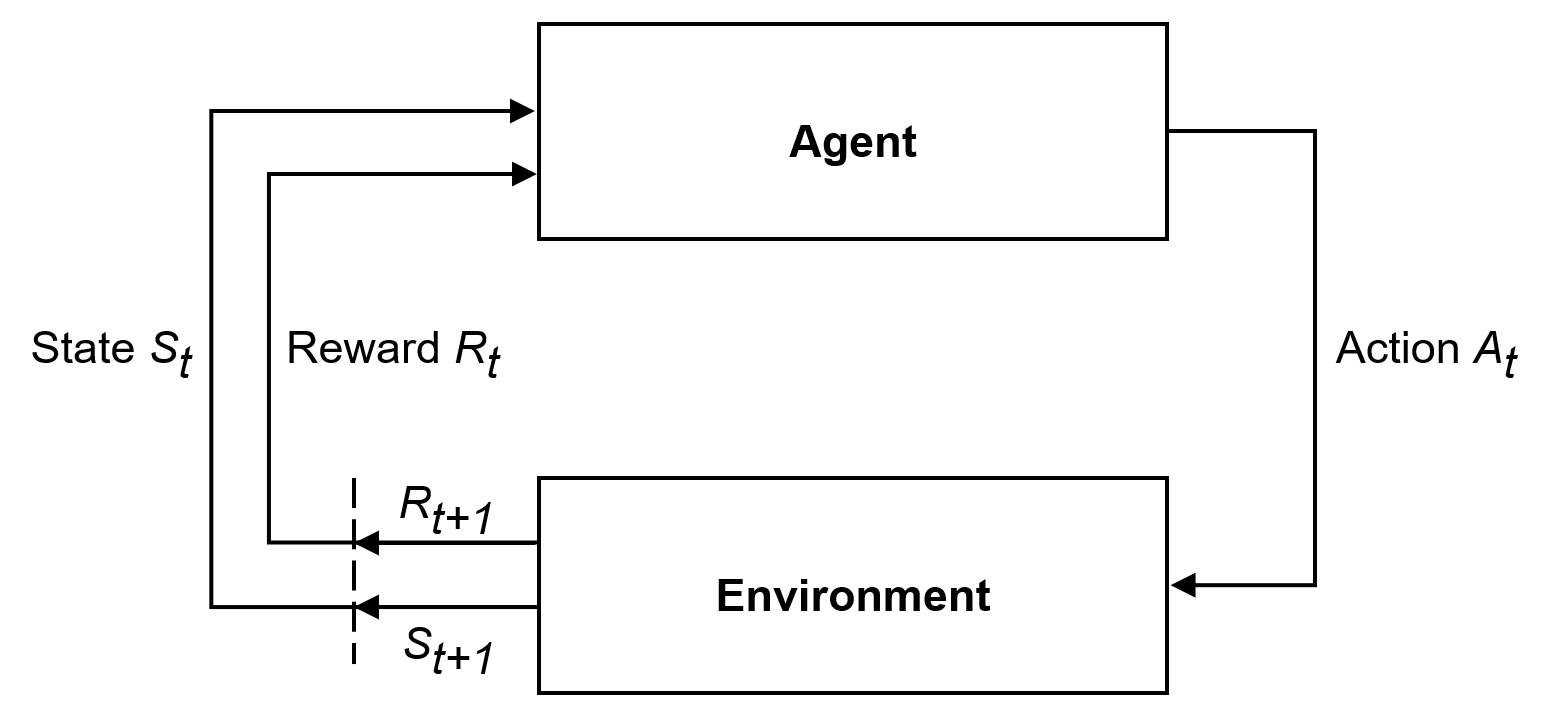
\includegraphics[height=5cm]{img/agent-env_MDP.png}
\caption{MDP framework (based on \textcite{SuttonBarto_2018})}
\label{fig:interaction-MDP}
\end{figure}

This framework can be generalised further (as shown in \autoref{fig:interaction-POMDP}) to also describe Partially Observable MDPs (\glsunset{pomdp}\gls{pomdp}) \parencite{silver2015}. \glspl{pomdp} are cases in which the agent is unable to fully observe the state of the environment.
In this framework, $S_t^e$ denotes the environment state. The observation $O_t$ is the information about the environment state that is emitted to the agent. In a \gls{pomdp}, the agent's internal representation of the state $S^a_t$ differs from $S_t^e$ and is constructed for example as a function of the previous state $S^a_{t-1}$ and the observation $O_t$. An \gls{mdp} is a special case where $O_t=S_t^e=S^a_t$.

\begin{figure}[H]
\centering
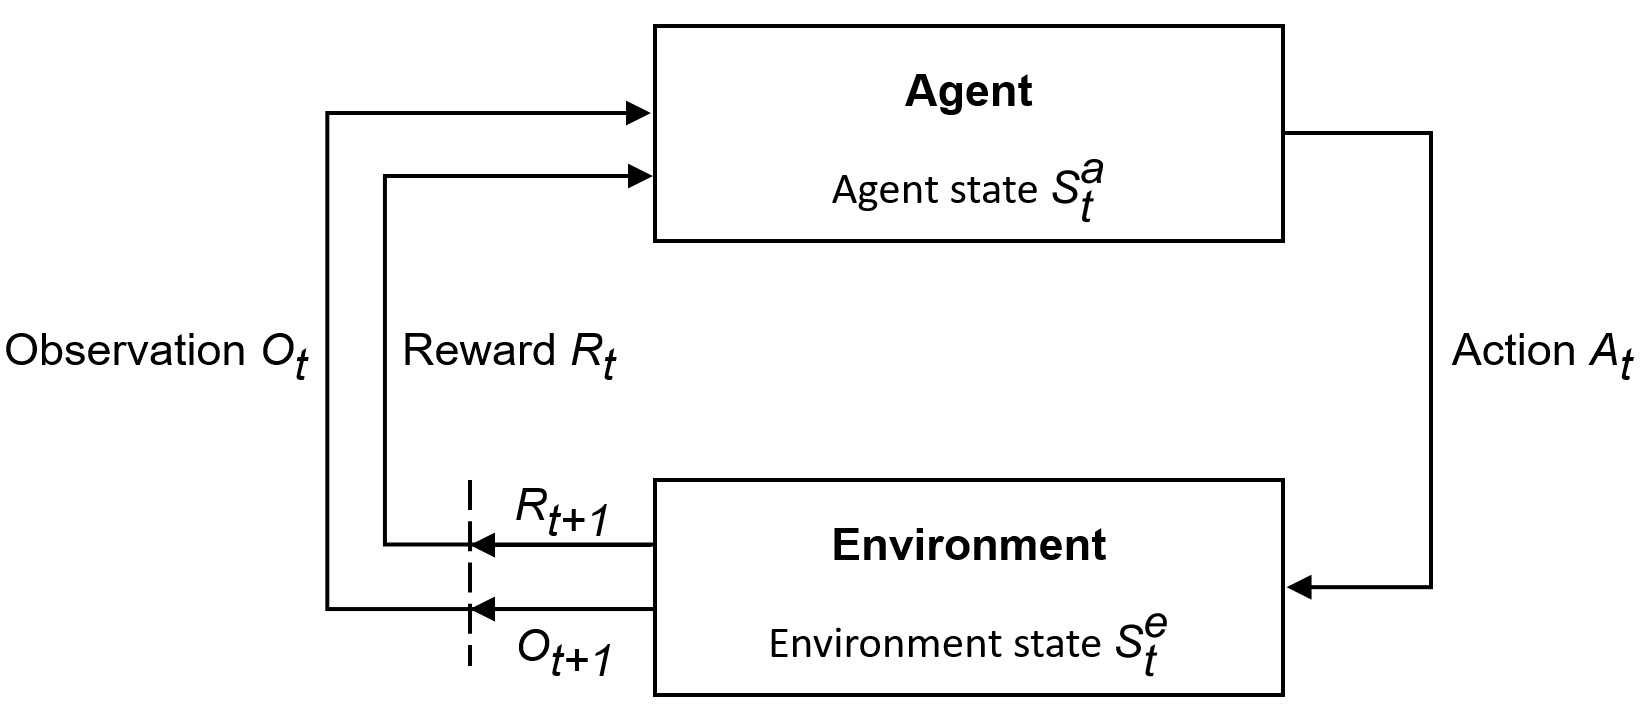
\includegraphics[height=5cm]{img/agent-env_POMDP.png}
\caption{POMDP framework (based on \textcite{silver2015})}
\label{fig:interaction-POMDP}
\end{figure}

\subsection{Policies}

The behaviour of an agent is defined by a policy $\pi$
\parencite{SuttonBarto_2018}. The policy is defined by the probability distribution of actions given the state (\autoref{equ:policy}). In other words, the policy determines which action the agent executes at each time step.

\begin{equation}
\label{equ:policy}
\pi(a|s) = Pr\lbrace A_t=a | S_t = s\rbrace
\end{equation}

%\subsection{On-Policy vs. Off-Policy Methods}

During the training of an \gls{rl} agent, there is a distinction between the behaviour policy and the target policy \parencite{Wang_2022}. The behaviour policy is the policy that the agent acts upon when generating training data. The target policy is the policy that is optimised through learning and should maximise the returns. 

With this distinction, \gls{rl} algorithms can be classified as either on-policy or off-policy \parencite{Wang_2022}. On-policy methods use the target policy as the behaviour policy. This means that in each round of optimisation, the target policy is used to generate the training samples. At the end of each round, these samples are discarded to avoid optimising on old policies.
In off-policy methods on the other hand, the target and behaviour policies differ. The samples are generated by the behaviour policies and are stored in a buffer. Samples from this buffer are then used to update the target policy.

Due to the fact that samples in the buffer can be re-used, off-policy methods have a higher data efficiency compared to on-policy methods \parencite{Wang_2022}. However, off-policy methods have more variance and converge slower than on-policy methods \parencite{SuttonBarto_2018}. 

\subsection{Value Functions}

The aim of an \gls{rl} agent is to maximise the total reward, which is also referred to as the return $G_t$ \parencite{SuttonBarto_2018}. This means that an agent should not only consider the immediate reward that is gained by taking an action, but future rewards should be considered as well. In \gls{rl}, the discounted return (\autoref{equ:disc_ret}) is usually considered. Here, the discount factor $\gamma \in [0, 1]$ weighs the importance of future rewards. If $\gamma = 0$, then the agent is only interested in the immediate rewards. As $\gamma$ increases, so does the importance of future rewards and the agent becomes increasingly far-sighted.

\begin{equation}
\label{equ:disc_ret}
G_t = R_{t+1} + \gamma R_{t+2} + \gamma^2 R_{t+3} + \gamma^3 R_{t+4} + ... = \sum^{\infty}_{k=0} \gamma^k R_{t+1+k}
\end{equation}

The expected return can be used to determine how good it is for an agent to be in a given state. This is quantified by the state-value-function $V(s)$, which gives the expected return when the agent starts in the state $s$ (\autoref{equ:state_val}). The higher the value, the better it is to be in the state. Using the Bellman equation, this can also be expressed in terms of the immediate reward and the discounted value of the next state (\autoref{equ:state_val_bellman}).

\begin{equation}
\label{equ:state_val}
V(s)= \mathbb{E}[G_t | S_t=s]
\end{equation}
\begin{equation}
\label{equ:state_val_bellman}
V(s)= \mathbb{E}[R_{t+1}+\gamma V(S_{t+1})| S_t=s]
\end{equation}

Likewise, the expected return can be used to determine how good an action is in a given state. The action-value function $Q(s, a)$ gives the expected return when the agent starts in the state $s$ and takes an action $a$ (\autoref{equ:action_val}). The higher the value, the better it is to take the action when in that state. This can also be transformed using the Bellman equation, which results in \autoref{equ:action_val_bellman}.

\begin{equation}
\label{equ:action_val}
Q(s, a)= \mathbb{E}[G_t | S_t=s, A_t=a]
\end{equation}
\begin{equation}
\label{equ:action_val_bellman}
Q(s, a)= \mathbb{E}[R_{t+1}+\gamma Q(S_{t+1}, A_{t+1}) | S_t=s, A_t=a]
\end{equation}

An optimal value function $V_*(s)$ or $Q_*(s, a)$ is defined as the value function that is obtained when following an optimal policy $\pi_*$ (Equations \ref{equ:optimal_state_val} and \ref{equ:optimal_action_val}). The optimal policy is the policy that maximises the return for all states.

\begin{equation}
\label{equ:optimal_state_val}
V_*(s)=\max_{\pi} V_\pi(s)
\end{equation}
\begin{equation}
\label{equ:optimal_action_val}
Q_*(s, a)=\max_{\pi} Q_\pi(s, a)
\end{equation}

\subsection{Reinforcement Learning Approaches}

One distinction that can be made when categorising \gls{rl} approaches is model-based vs. model-free \parencite{SuttonBarto_2018}. Model-based approaches require a model of the environment, which can be used to predict how the environment will behave. These models are used to evaluate potential next actions by considering all possible outcomes before they happen. This is referred to as planning.
% Examples for model-free algorithms are ...

Model-free approaches, on the other hand, learn through trial-and-error and do not require a model of the environment \parencite{SuttonBarto_2018}. Such approaches can be further classified as value-based methods, policy gradient methods or actor-critic methods.

Value-based algorithms aim to estimate the optimal value function \parencite{Wang_2022}. The optimal policy is implicitly given by the value function. For example, the target policy might be to behave greedily with respect to $Q_*(s, a)$. Examples for these algorithms are Q-Learning \parencite{Watkins_1992} and Deep Q-Learning (\gls{dqn}) \parencite{Mnih_2015}.

Policy gradient algorithms aim to optimise the target policy directly \parencite{Wang_2022}. Here, the parameterised policy $\pi_\theta(a|s)=Pr(a|s, \theta)$ is updated based on the gradient of a policy objective function $J(\theta)$. According to the policy gradient theorem, this can be calculated using \autoref{equ:policy-grad} \parencite{silver2015}. The benefit of this approach is that the policy does not become deterministic and therefore continues to allow for exploration \parencite{SuttonBarto_2018}. An example of a policy gradient algorithm is REINFORCE \parencite{Williams_1992}.

\begin{equation}
\label{equ:policy-grad}
\nabla_\theta J(\theta)=\mathbb{E}_{\pi_\theta}[Q_{\pi_\theta}(s, a)\cdot\nabla_\theta log\pi_\theta(a|s)]
\end{equation}

Actor-critic methods are methods that learn a policy and a value function at the same time \parencite{Wang_2022}. The actor generates policies, interacts with the environment and updates the target policy using the policy gradient. The critic learns the state-value function $V(s)$, action-value function $Q(s, a)$ or the advantage function $A(s, a)$ and uses this to evaluate the actor's policy. The advantage is defined in \autoref{equ:advantage} and represents the relative value of taking an action in a given state. This can be used instead of $Q(s, a)$ when calculating the gradient of the objective function (\autoref{equ:policy-grad}) to reduce the variance of the gradients.

\begin{equation}
\label{equ:advantage}
A(s, a)=Q(s, a)-V(s)
\end{equation}

%Value-Based methods: learn q values. Implicit policy is to select avtion with highest value. Doesnt require knowledge about environment. E.g. Q-learning (constructs table of q values, not scalable), DQN (uses function approximation to represent q-values usually NN).

%Policy-based methods: learn policy

%Actor-Critic methods:

%\begin{figure}[H]
%\centering
%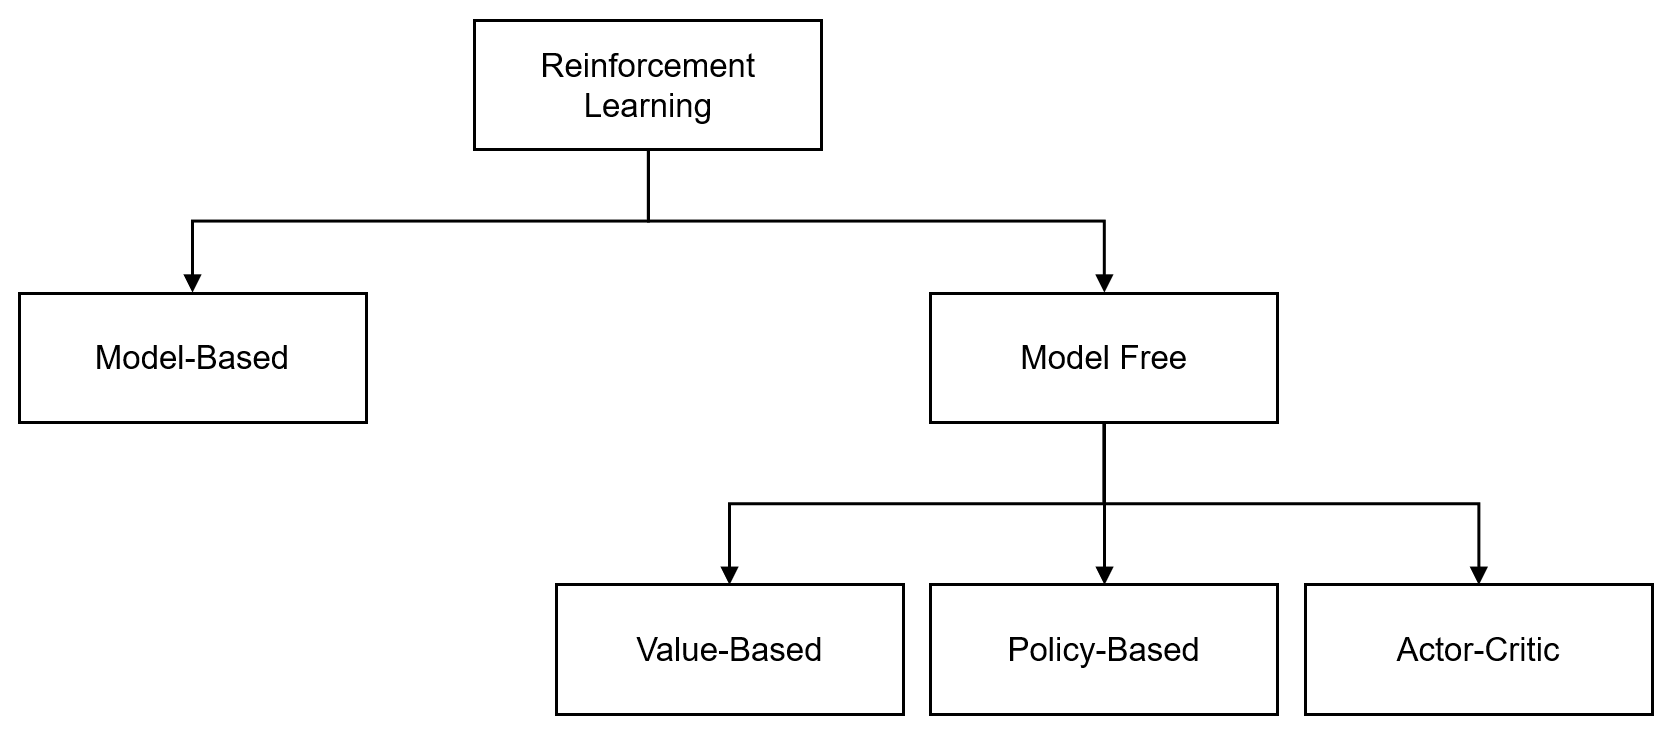
\includegraphics[height=5cm]{img/rl-approaches.png}
%\caption{Taxonomy of RL approaches}
%\label{fig:rl-approaches}
%\end{figure}






\section{Continual Learning}

Definition

\subsection{Continual Learning Problems}

Classification of problems

non-stationarity drivers etc.

\subsection{Continual Learning Agents}

ideal attributes of CL agent

CL Approaches

Explicit knowledge retention will be reviewed on more detail.

\subsection{Explicit Knowledge Retention}

\subsubsection{Latent Parameter Storage}

Definition

Discuss papers that do this

\subsubsection{Distillation Based}

Definition

Discuss papers that do this

\subsubsection{Rehearsal Based}

Definition

Discuss papers that do this


\section{Reinforcement Learning in Urban Traffic Control}